\section{Reconstruction and calibration of distance modulus using Deep Learning}
We construct the RNN+BNN network and train it with the package TensorFlow2\cite{tensorflow2015-whitepaper}. For clarity, we present the corresponding hyperparameters in Figure 1 and list the steps to reconstruct data with our network as follow: (a) Data processing. The scale of data has an effect on training. Hence, we normalize the distance moduli of the sorted Pantheon data and re-arrange $\mu-z$ as sequences with the step number t = 4. (b) Building RNN. We build RNN with three layers, i.e. an input layer, a hidden layer and an output layer as described in Figure 1. The first two layers are constructed with the LSTM cells of 100 neurons. The redshifts $z_{<t>}$ and the corresponding distance moduli $\mu_{<t>}$ are the input and output vectors, respectively. We employ the Adam optimizer to minimize the cost function MSE and train the network 1000 times. (c) Building BNN. We set the dropout rate to 0 in the input layer to avoid the lost of information, and to 0.2 in the second layer as well as the output layer (Bonjean 2020; Mangena et al. 2020). We execute the trained network 1000 times to obtain the distribution of distance moduli
\subsection{Training}
We train the neural network using pantheon data. The pantheon data is split into train and test data in equal size randomly. 512 datapoints are used for training and remaiing for testing. The network architecture is described in previous section. We use meansquared error loss and adam optimizer, with early stopping technique to prevent overfitting. Dropout technique with $dropout_rate$ = 0.2. The hyperparameters used are $batch_size$ = 10, $learning_rate$ = 1e-3, $patience$ = 5.
\begin{figure}[h]
	\centering
	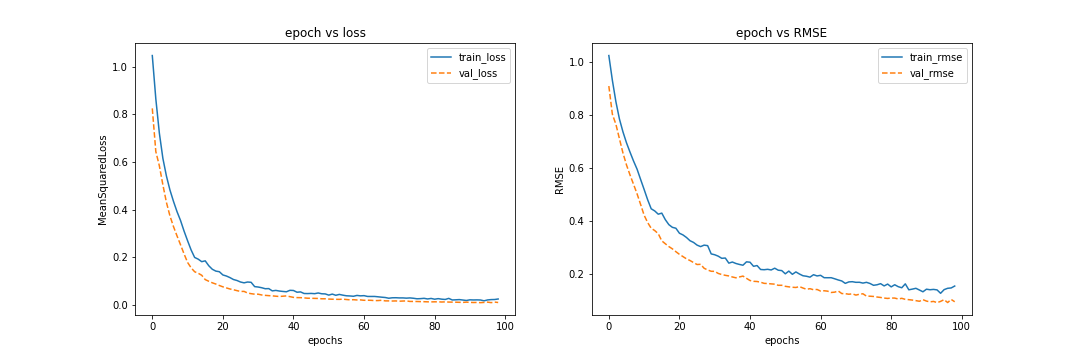
\includegraphics[width=\textwidth]{pantheon/lstm/05_epoch_vs_loss.png}
	\caption{Loss curve}
	\label{fig:loss_curve}
\end{figure}
\begin{figure}[h]
	\centering
	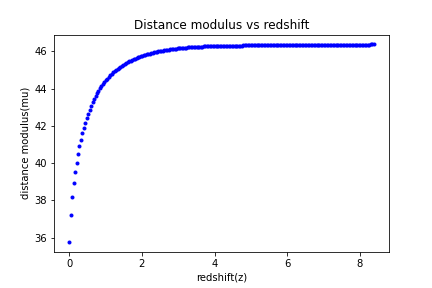
\includegraphics[width=\textwidth]{pantheon/lstm/06_sample_reconstruction.png}
	\caption{Loss curve}
	\label{fig:reconstruction}
\end{figure}
\subsection{Testing redshift dependence of luminosity correlations}
\begin{table}[H]
\centering
\begin{tabular}{|c|c|c|c|c|c|c|c|c|}
\hline
Correlation & sample & N & a & $a_err$ & b & $b_err$ & $\sigma$ & $\sigma_{int}$\\
\hline
\multirow{3}{*}{$T_{lag}-L$} & low-z & 37 & 52.1 & 0.1 & -0.77 & 0.15 & 0.49 & 0.08\\
\cline{2-9}
 & high-z & 32 & 52.37 & 0.07 & -0.6 & 0.12 & 0.29 & 0.07\\
\cline{2-9}
 & All-z & 69 & 52.22 & 0.06 & -0.7 & 0.1 & 0.42 & 0.05\\
\hline
\multirow{3}{*}{$V-L$} & low-z & 47 & 52.12 & 0.25 & 0.65 & 0.36 & 0.91 & 0.13\\
\cline{2-9}
 & high-z & 57 & 52.63 & 0.18 & 0.25 & 0.17 & 0.63 & 0.07\\
\cline{2-9}
 & All-z & 104 & 52.34 & 0.13 & 0.46 & 0.14 & 0.75 & 0.07\\
\hline
\multirow{3}{*}{$E_{peak}-L$} & low-z & 50 & 51.89 & 0.09 & 1.43 & 0.18 & 0.59 & 0.07\\
\cline{2-9}
 & high-z & 66 & 52.23 & 0.05 & 1.09 & 0.14 & 0.34 & 0.05\\
\cline{2-9}
 & All-z & 116 & 52.05 & 0.05 & 1.35 & 0.12 & 0.5 & 0.04\\
\hline
\multirow{3}{*}{$E_{peak}-E_{\gamma}$} & low-z & 12 & 50.66 & 0.09 & 1.47 & 0.2 & 0.25 & 0.09\\
\cline{2-9}
 & high-z & 12 & 50.53 & 0.13 & 1.37 & 0.43 & 0.39 & 0.16\\
\cline{2-9}
 & All-z & 24 & 50.61 & 0.06 & 1.45 & 0.16 & 0.25 & 0.07\\
\hline
\multirow{3}{*}{$T_{RT}-L$} & low-z & 39 & 52.68 & 0.13 & -1.3 & 0.19 & 0.48 & 0.07\\
\cline{2-9}
 & high-z & 40 & 52.61 & 0.09 & -0.74 & 0.17 & 0.39 & 0.06\\
\cline{2-9}
 & All-z & 79 & 52.62 & 0.07 & -1.08 & 0.12 & 0.44 & 0.04\\
\hline
\multirow{3}{*}{$E_{peak}-E_{iso}$} & low-z & 40 & 52.57 & 0.1 & 1.55 & 0.2 & 0.6 & 0.08\\
\cline{2-9}
 & high-z & 61 & 52.74 & 0.06 & 1.2 & 0.15 & 0.4 & 0.04\\
\cline{2-9}
 & All-z & 101 & 52.65 & 0.05 & 1.42 & 0.12 & 0.49 & 0.04\\
\hline
\end{tabular}
\caption{A test caption}
\label{table_pantheon_lstm}
\end{table}


\begin{figure}[H]
	\centering
	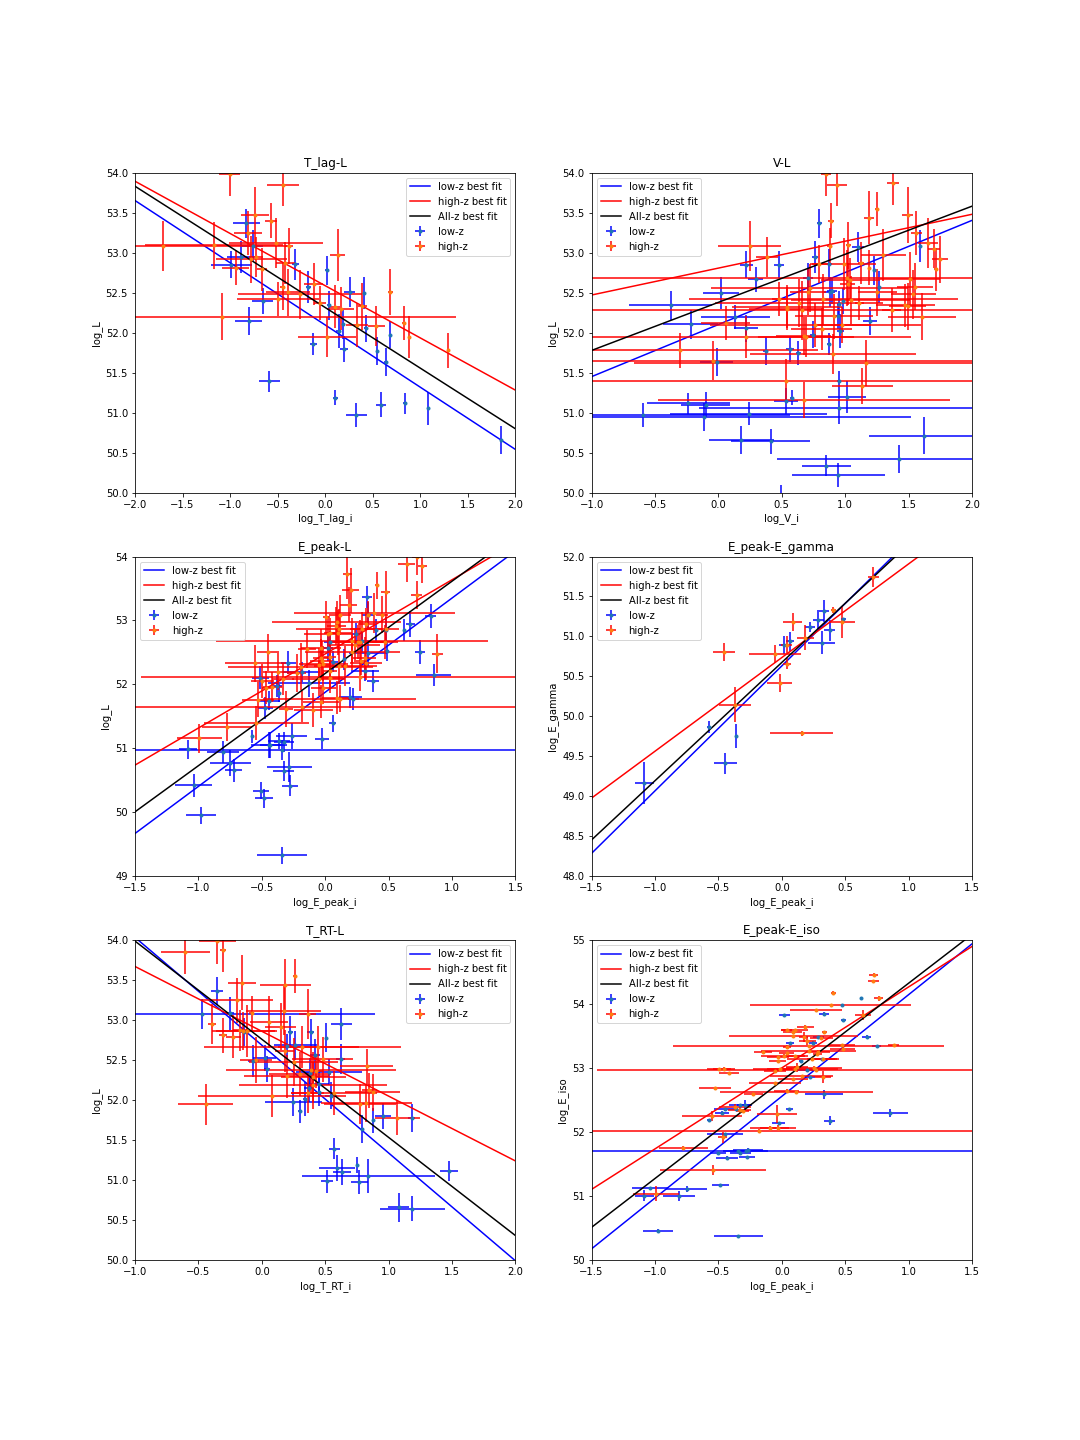
\includegraphics[width=\textwidth]{pantheon/lstm/15_correlatin.png}
	\caption{Luminsosity correlations best fit}
	\label{fig:correlation_lstm}
\end{figure}

\subsection{Calibrating distance modulus from $E_{peak}-E_{gamma}$ relation}
\begin{figure}[H]
	\centering
	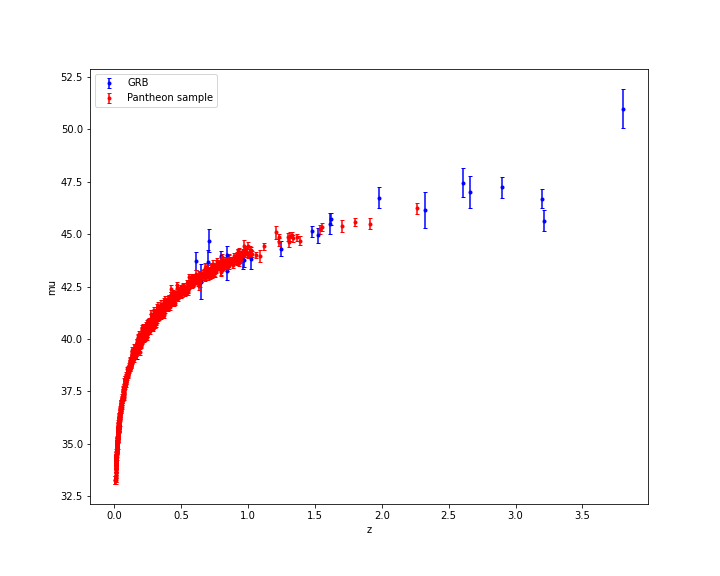
\includegraphics[width=\textwidth]{pantheon/lstm/16_GRB_reconstruction.png}
	\caption{GRB Hubble Diagram}
	\label{fig:HD_GRB_GP}
\end{figure}
\subsection{Constraints on dark energy}
\begin{figure}[h]
	\centering
	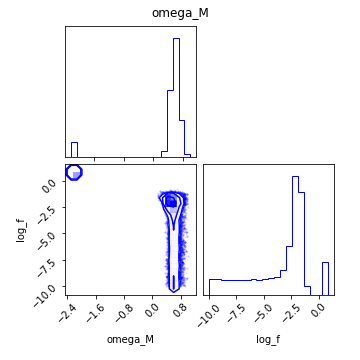
\includegraphics[width=\textwidth]{pantheon/lstm/18_omega_M_corner_plot.png}
	\caption{GRB Hubble Diagram}
	\label{fig:OmegaM_lstm}
\end{figure}